\chapter{Standard Templates Library}
% \section*{17 - Ottobre}
The goal of STL is to represent algorithms in as general form as possible without compromising efficiency.
There is an extensive use of \textbf{templates}, \textbf{overloading}\note{Same function name, the algorithm to be executed is determined by the type of the arguments} and \ul{\textbf{iterators}},
which are used for decoupling algorithms from containers,
and can be seen as an \ul{abstraction of pointers}.\\
STL is very different from the \textit{Java Collection Library} since it does \textbf{not} use \textit{dynamic binding} and is \textbf{not} \textit{object oriented};
instead the STL uses only \textit{static binding} and \textit{inlining}.

\section{Main Entities}
\begin{itemize}
   \item \textbf{Container} collection of \textit{typed} objects
   \item \textbf{Iterator} Generalization of pointer or address;
   used to step through the elements of collections
   \item \textbf{Algorithm} initializing, sorting, searching, and transforming contents of containers
   \item \textbf{Adaptor} Convert from one form to another e.g. iterator from updatable container; or stack from list
   \item \textbf{Function Object} Form of closure (class with "operator()" defined)
   \item \textbf{Allocator} encapsulation of a memory pool
\end{itemize}

\begin{figure}[h]
   \centering
   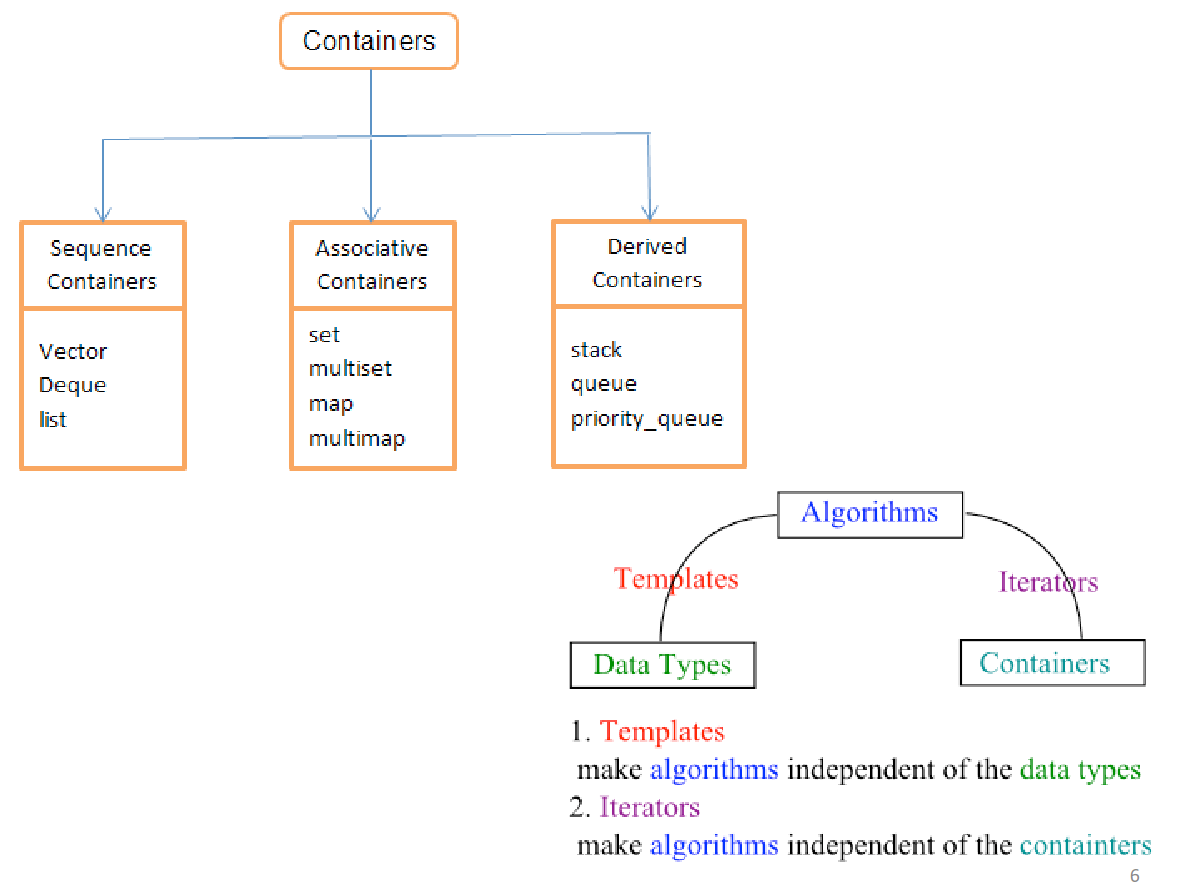
\includegraphics[width=0.7\textwidth]{images/STL_containers.png}
   \label{fig:STL_containers}
\end{figure}

\section{Iterators}
Since algorithms cannot be used \textit{directly} on different kinds of collections,
Iterators come in handy by providing a \textbf{uniform}, \textbf{linear} access to elements of different collections.

In \textbf{Java} iterators are supported by the \textit{JCF}\footnote{\textit{Java Collection Framework}} through the interface \lstinline|Interface<T>|.
They are related to an \textbf{instance} of a class and are usually defined as \textit{nested classes},
more precisely \textit{non-static private member classes}.\\
Collections equipped with iterators must \lstinline|implements Iterable<T>| interface.

\section*{18 - Ottobre}

In \textbf{C++} there is no \lstinline|next/hasNext()| function, standard \lstinline|++ --| operators are used instead.\\
\lstset{language=C++}
In case of \textit{arrays} pointers can be trivially used,
since \lstinline|int v[]| is no different \lstinline|int *v|\footnote{At least from an "accessing values" point of view, there are some differences in terms of static/dynamic allocation of memory.}.
In the case of \lstinline|vector| instead, an actual \textit{iterator} may be instantiated,
but the operator \lstinline|++| stays the same.
\begin{lstlisting}
   vector<int> vec;
   vector<int>::iterator v = vec.begin();
   while( v != vec.end()) {
      cout << "value of v = " << *v << endl;
      v++;
   }
\end{lstlisting}

Every class in C++ has its own iterator;
more specifically, containers define and expose a type named iterator in the container's \textbf{namespace},
allowing the semantic value of \lstinline|iterator| to change according to the context.

\subsection{C++ iterators implementation}
Typically iterators are implemented as \lstinline|struct| and provide a visit of the container,
retaining information about the \textbf{state} of the visit, e.g. pointer to next element, remaining elements, and so on.
Note that in case of \textit{trees} or \textit{graphs} the visit's state may not be trivial to be represented.
\begin{lstlisting}
  template <class T>
  struct v_iterator {
    T* v;
    int sz;
    v_iterator(T* v, int sz) : v(v), sz(sz) {}
    // != implicitly defined
    bool operator==(v_iterator& p) { return v == p->v; }
    T operator*() { return *v; }
    v_iterator& operator++() {  // Pre-increment
      if (sz)
        ++v, --sz;
      else
        v = NULL;
      return *this;
    }
    v_iterator operator++(int) {  // Post-increment!
      v_iterator ret = *this;
      ++(*this);  // call pre-increment
      return ret;
    }
  };
\end{lstlisting}

\setlength{\heavyrulewidth}{1.5pt}
\setlength{\abovetopsep}{4pt}
\begin{table}[!htbp]
  \centering
  \begin{tabular}{c|c|c|c}
    \toprule
    & \multicolumn{3}{c}{\textit{insert/erase}}\\
    \textbf{Container} & \textbf{beginning} & \textbf{middle} & \textbf{end} \\
    \midrule
    \textit{vector}  & linear              & linear    & amortized constant\\
    \textit{list}    & constant            & constant  & constant\\
    \textit{deque}   & amortized constant  & linear    & amortized constant\\
    \hline
  \end{tabular}
  \caption{\textbf{Guaranteed} time complexity for iterators}
\end{table}

To achieve transparency to third-party algorithms STL assumes \textit{constant} time for every operation, and allows 5 types of operators:
\begin{itemize}
  \item \textit{Formard iterators} only dereference and pre/post increment
  \item \textit{Input (and Output) iterators} same as \textit{formard iterators} but with possible issues when dereferencing
  \item \textit{Bidirectional iterators} dereference, pre/post increment and decrement
  \item \textit{Random access iterators} same as Bidirectional but allow also integer sum $(p + n)$ and difference $(p - q)$
\end{itemize}
Each category defines only the functions which take constant time. Not all iterators are defined for all
containers, e.g. since \textit{random access} takes \textit{linear} time on lists,
there is no \textit{random access} iterator on \textit{lists}.
\note{Any C++ pointer type, T*, obeys all the laws of the random access iterator category}

\subsection{Invalidation}
When a container is \textit{modified},
iterators \textit{may} become \textbf{invalid}:
no "exception" is thrown,
iterators can still be used,
but their behaviour is \textbf{undefined}.
\textit{\textbf{Not} every operation} invalidates iterators,
\ul{it depends on the operation and on the container}.
For example, inserting an element in a \lstinline|list| allows all iterators to remain valid, while inserting an element in a \lstinline|vector| invalidates all of them, since reallocation is necessary.
\nl

The main limiting aspect of STL's iterators is that they provide a \textbf{linear view} of the container,
allowing the definition of operations only on one-dimensional containers;
thus, if it is needed to access the organization of the container (e.g. tree custom visist), the only way-to-go is to define a custom iterator which behaves as desired.

\section{C++ specific features}

\subsection{Inheritance}
STL relies on typedefs combined with namespaces to
implement genericity, the programmer always refers to \lstinline|container::iterator| to know the type of the iterator.
Note that there is \ul{no relation among iterators for different containers }(!), if not a semantically abstract one.
The reason for this is \textbf{performance}: 
without \textit{inheritance}, types are resolved at compile time and the compiler may produce better and optimized code.
On the other hand sacrificing inheritance may lead to
lower expressivity and lack of type-checking;
in fact, STL relies only on coding conventions:
when the programmer uses a wrong iterator the compiler complains of a bug in the library.

\subsection{Inlining}
C++ standard has the notion of \textbf{inlining} which is a form of semantic macros.
Inline methods should be available in header files
and can be labelled \textit{inline} or defined within class
definition, invocation on such methods is type-checked and then it is
replaced by the method body.
The compiler tends to (automatically?)
inline methods with small bodies and without iteration; 
it is able to determine types at compile
time and usually does inlining of function objects.

\lstset{language=C++}
\begin{lstlisting}
  template <class T>
  inline T sqr(T x) { return x * x; }
\end{lstlisting}

\lstset{style=javaBlockAnn}

\subsection{Memory management}
STL abstract from the specific memory model using a concept named \textbf{allocators}.
All the information about the memory model is
encapsulated in the \textbf{Allocator} class.
Each container is parametrized by such an allocator to let
the implementation be unchanged when switching
memory models.

\subsection{Potential Problems}
The problem may be error checking: 
almost all facilities of the compiler fail with STL resulting in lengthy error messages that ends with error within the library